\documentclass[11pt,a4paper]{article}
\usepackage[margin=1in]{geometry}
\usepackage[T1]{fontenc}
\usepackage[utf8]{inputenc}
\usepackage{graphicx}
\usepackage{hyperref}
\usepackage{enumitem}
\usepackage{float}
\usepackage{booktabs}
\usepackage{xcolor}
\usepackage{listings}

\lstset{
  basicstyle=\ttfamily\small,
  breaklines=true,
  frame=single,
  backgroundcolor=\color{gray!10},
}

\title{Air Quality Intelligence System\\[0.3em]
\large Advanced Database Management Systems --- Course Report}
\author{Péter Dobosi}
\date{\today}

\begin{document}
\maketitle

% ============================================================
\section{Team Information}

\begin{tabular}{@{}ll@{}}
\toprule
\textbf{Field} & \textbf{Value} \\
\midrule
Student & Péter Dobosi \\
Neptun code & DOP3BP \\
Course & Advanced Database Management Systems \\
Semester & 2025/26 Spring \\
Repository & \url{https://github.com/dobosipeter/advanced-data-warehouse-and-database-management-systems-submission} \\
Live system & \url{https://mw79on-demo.online} \\
API docs & \url{https://api.mw79on-demo.online/docs} \\
\bottomrule
\end{tabular}

% ============================================================
\section{System Architecture}

The system is a real-time air quality monitoring and alerting platform ingesting data
from the OpenAQ public API into a PostgreSQL database, processing it through triggers
and transactions, and exposing it via a FastAPI REST backend and Streamlit GUI.

\begin{figure}[H]
\centering
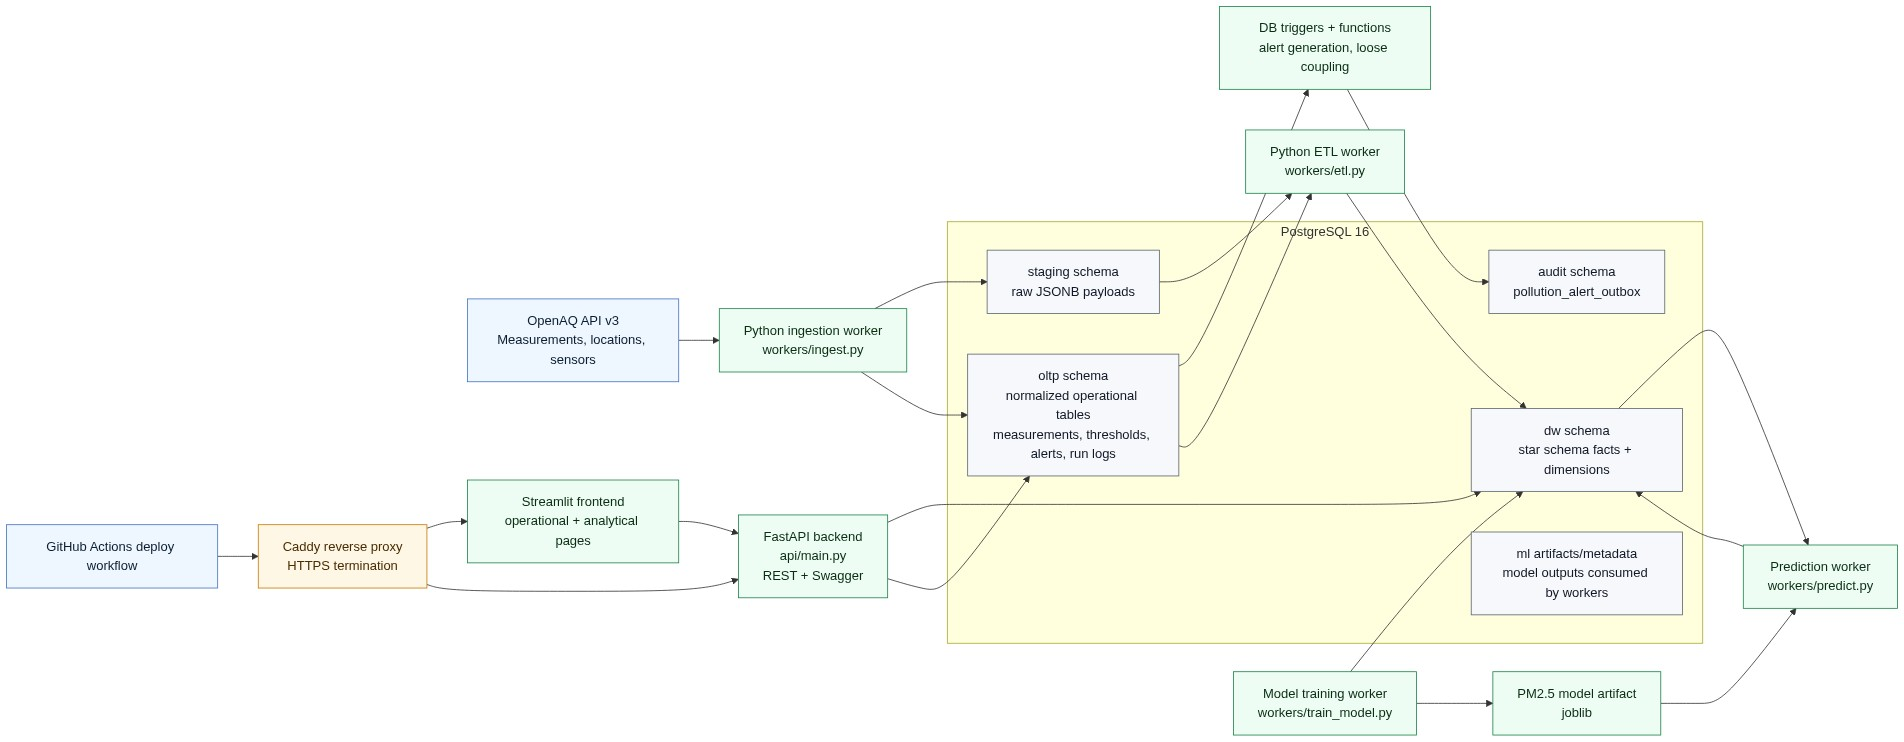
\includegraphics[width=\textwidth]{../../diagrams/system_architecture.png}
\caption{System architecture overview (emphasis on OLTP layer).}
\label{fig:architecture}
\end{figure}

\noindent Key DBMS-oriented components:
\begin{itemize}[nosep]
  \item \textbf{PostgreSQL 16} --- OLTP engine with schemas: \texttt{oltp}, \texttt{staging}, \texttt{audit}.
  \item \textbf{Triggers} --- automatic alert generation on measurement insert; outbox event enqueue on alert state change.
  \item \textbf{Transactions} --- all ingestion batches run inside explicit transactions with savepoints; failures roll back atomically.
  \item \textbf{Constraints} --- CHECK, UNIQUE, FOREIGN KEY, and cross-column constraints on every table.
  \item \textbf{Partitioning} --- \texttt{measurement\_raw} is range-partitioned by \texttt{measured\_at} (monthly).
  \item \textbf{Indexing} --- B-tree indexes on foreign keys, composite indexes on hot query paths.
  \item \textbf{Backup} --- scripted \texttt{pg\_dump} with rotation and optional off-site upload.
  \item \textbf{FastAPI} --- RESTful API with OpenAPI/Swagger auto-docs.
  \item \textbf{Streamlit} --- Operational GUI for threshold management, alert review, and system monitoring.
\end{itemize}

% ============================================================
\section{Functional Specification}

The operational (DBMS) layer provides the following features:

\begin{enumerate}[nosep]
  \item \textbf{Data Ingestion} --- Incremental and initial bulk load from OpenAQ v3 API via Python worker.
  \item \textbf{Threshold Management} --- CRUD for per-city, per-pollutant alert rules with severity levels (low / moderate / high / critical).
  \item \textbf{Automatic Alert Generation} --- PostgreSQL trigger fires on every new measurement, matches against active threshold rules, and inserts an alert row.
  \item \textbf{Outbox Pattern} --- A second trigger enqueues alert lifecycle events into an audit outbox table for downstream consumers.
  \item \textbf{Alert Review Workflow} --- Operators can transition alerts through open → reviewed → closed with notes.
  \item \textbf{Transaction Safety} --- Ingestion uses explicit transactions; partial failures are rolled back without corrupting existing data.
  \item \textbf{Partitioning} --- Monthly range partitions on the measurement table enable partition pruning on time-range queries and simplify archival.
  \item \textbf{Indexing} --- Targeted indexes accelerate JOIN-heavy API queries (measurements by sensor, alerts by status, thresholds by city/parameter).
  \item \textbf{Backup \& Maintenance} --- Cron-driven \texttt{pg\_dump} with configurable retention and VACUUM/ANALYZE scheduling.
  \item \textbf{REST API} --- FastAPI backend exposes health, locations, measurements, alerts, thresholds, ingestion runs, and predictions.
  \item \textbf{Operational GUI} --- Streamlit dashboard with pages for station exploration, threshold editing, alert management, and system status.
  \item \textbf{CI/CD Deployment} --- GitHub Actions workflow deploys changes to the Hetzner VM automatically on push to \texttt{main}.
\end{enumerate}

% ============================================================
\section{Logical Data Model (OLTP)}

The OLTP schema (\texttt{oltp}) contains the following tables:

\begin{table}[H]
\centering
\small
\begin{tabular}{@{}lll@{}}
\toprule
\textbf{Table} & \textbf{Primary Key} & \textbf{Purpose} \\
\midrule
\texttt{ingestion\_run\_log} & \texttt{ingestion\_run\_id} & Track each pipeline run (status, counts, errors) \\
\texttt{parameter} & \texttt{parameter\_id} & Pollutant definitions (pm25, pm10, no2, o3, \ldots) \\
\texttt{location} & \texttt{location\_id} & Monitoring stations with coordinates and metadata \\
\texttt{sensor} & \texttt{sensor\_id} & Physical sensors linking locations to parameters \\
\texttt{measurement\_raw} & \texttt{(measurement\_id, measured\_at)} & Raw observations (partitioned by month) \\
\texttt{threshold\_rule} & \texttt{threshold\_rule\_id} & Alert threshold definitions per city/pollutant/level \\
\texttt{pollution\_alert} & \texttt{pollution\_alert\_id} & Generated alerts referencing measurements \& rules \\
\bottomrule
\end{tabular}
\caption{OLTP tables.}
\end{table}

\noindent Supporting schemas:
\begin{itemize}[nosep]
  \item \texttt{staging.raw\_api\_response} --- stores raw JSON API responses for auditability.
  \item \texttt{audit.pollution\_alert\_outbox} --- event sourcing table for alert lifecycle events.
\end{itemize}

\subsection*{Key Relationships}

\begin{itemize}[nosep]
  \item \texttt{sensor} → \texttt{location} (many-to-one)
  \item \texttt{sensor} → \texttt{parameter} (many-to-one)
  \item \texttt{measurement\_raw} → \texttt{sensor} (many-to-one)
  \item \texttt{measurement\_raw} → \texttt{ingestion\_run\_log} (many-to-one, nullable)
  \item \texttt{pollution\_alert} → \texttt{measurement\_raw} (composite FK)
  \item \texttt{pollution\_alert} → \texttt{threshold\_rule} (many-to-one)
\end{itemize}

% ============================================================
\section{Technologies Used}

\begin{table}[H]
\centering
\begin{tabular}{@{}ll@{}}
\toprule
\textbf{Technology} & \textbf{Role} \\
\midrule
PostgreSQL 16 & RDBMS (OLTP + DW + audit schemas) \\
Python 3.12 & Worker scripts, API, frontend \\
FastAPI & REST API with automatic OpenAPI docs \\
Streamlit & Operational + analytical dashboards \\
Docker Compose & Container orchestration \\
Caddy & Reverse proxy with automatic HTTPS \\
GitHub Actions & CI/CD pipeline (SSH deploy) \\
Hetzner Cloud & Production VM (Ubuntu 24.04) \\
\bottomrule
\end{tabular}
\caption{Technology stack.}
\end{table}

\subsection*{Notable PostgreSQL Features Demonstrated}

\begin{itemize}[nosep]
  \item \textbf{PL/pgSQL triggers} (alert generation, outbox enqueue)
  \item \textbf{Range partitioning} (monthly measurement partitions)
  \item \textbf{CHECK constraints} with cross-column validation
  \item \textbf{Composite primary/foreign keys}
  \item \textbf{JSONB columns} for flexible raw payload storage
  \item \textbf{Explicit transactions with savepoints} in ingestion scripts
  \item \textbf{pg\_dump} for automated backup and recovery
\end{itemize}

\end{document}
